\section{Machine Learning}%
\label{sec:machine_learning}

Methods of multivariate analysis (MVA) have been used for decades in HEP to
maximise the insights gained from experimental data. Previously, these analyses
were often performed by hand, a difficult and time-consuming process,
particularly when working with high-dimensional data. Over the past decade,
automated approaches of MVA have become increasingly popular, freeing up
researchers and frequently outperforming handcrafted solutions. This automation
is achieved by algorithms that construct predictive models using samples of
training data, a process referred to as \emph{machine learning}.

Arguably the most common type of machine learning used in HEP falls under the
category of \emph{supervised learning}. The goal of supervised learning is to
build models that predict an outcome~$\myvec{Y}$ using a set of
predictors~$\myvec{X}$ by learning from a sample of labelled training
data~$\{ (\myvec{x}_i, \myvec{y}_i) \}_{i=1}^{N}$. Depending on the type of
outcome a distinction between classification (categorical outcomes) and
regression (continuous outcomes, count outcomes, etc.) is made. Supervised
learning is particularly applicable in HEP, since large amounts of labelled
training data can be generated using Monte Carlo (MC) simulation.
% , the simulations being heavily tuned to experimental observations to
% accurately represent the data-generating processes.
Nowadays, the state-of-the-art solutions to many tasks in HEP, for example
particle identification, are based on machine learning.

This section gives an overview of the machine learning algorithms used in this
thesis, specifically focusing on algorithms for solving binary classification
tasks. \Cref{sec:bdt} introduces \emph{boosted decision trees}, which are used
in \Cref{sec:dihiggs,sec:higgs_self_coupling} for signal-background
discrimination in the search for non-resonant \HH production. The basic
principles of \emph{neural networks} are introduced
in~\Cref{sec:neural_networks}, including a discussion of an architecture
referred to as \emph{recurrent neural networks}. Neural networks are used for
the identification of hadronic \taulepton decays in \Cref{sec:tauid}, as well as
for the search for resonant \HH production in~\Cref{sec:dihiggs}.


\subsection{Boosted Decision Trees}%
\label{sec:bdt}

Boosted decision trees (BDT) are models used for classification and regression
consisting of ensembles of \emph{decision trees}. These ensembles are created
using an algorithm called \emph{boosting}, which iteratively fits shallow
decision trees
% --or in general, any weak learning algorithm--
to altered versions of the training data. The training data is modified at every
iteration to emphasise prediction errors made by previous boosting
iterations. Finally, the predictions of the ensemble of trees are combined with
the goal of providing superior classification/regression performance compared to
a single decision tree. The following sections discuss the application of
decision trees to regression tasks (regression trees), as well as a
\emph{gradient boosting} algorithm that builds ensembles of regression trees to
perform binary classification.

% In the following, a description of one of the BDT algorithms implemented in
% \textsc{TMVA}~\cite{TMVA} is given, which is later used in the search for
% Higgs boson pair production.

\subsubsection{Decision Trees for Regression}

% Classification and regression trees~\cite{Breiman:1984jka,hastie09}, hereafter
% collectively referred to as \emph{decision trees}, are used as the basis for
% BDT.
A decision tree partitions an $n$-dimensional space with coordinates
$\myvec{x} = (x_1, \dots, x_n)$ by recursively performing binary splits along
the coordinate axes until a stopping criterion is
met~\cite{Breiman:1984jka,hastie09}. The resulting binary tree structure and
partitioning is illustrated in \Cref{fig:decision_tree} for a two-dimensional
example. A decision tree with $J$~leaf nodes splits the input space into
$J$~mutually disjoint subregions denoted by $R_j$ for $j = 1, \dots, J$. A
constant value $c_j$ is assigned to every region $R_j$ such that the prediction
of a decision tree for a point~$\myvec{x}$ can be expressed as
\begin{align*}
  h\bigl( \myvec{x}; \{c_j, R_j\}_{j=1}^{J} \bigr) = \sum_{j = 1}^{J} c_j \, \mathbf{1}(\myvec{x} \in R_j) \qquad \text{with} \qquad \mathbf{1}(\myvec{x} \in R_j) =
  \begin{cases}
    1, & \myvec{x} \in R_j \\
    0, & \text{else}
  \end{cases} \,\text{,}
\end{align*}
where $\{c_j, R_j\}_{j=1}^{J}$ fully characterises the decision
tree~\cite{hastie09}.

% An algorithm for growing a decision tree for a regression task, also referred
% to as a regression tree, is introduced, hereafter.\footnote{}

\begin{figure}[htbp]
  \centering

  \begin{subfigure}[b]{0.46\textwidth}
    \centering
    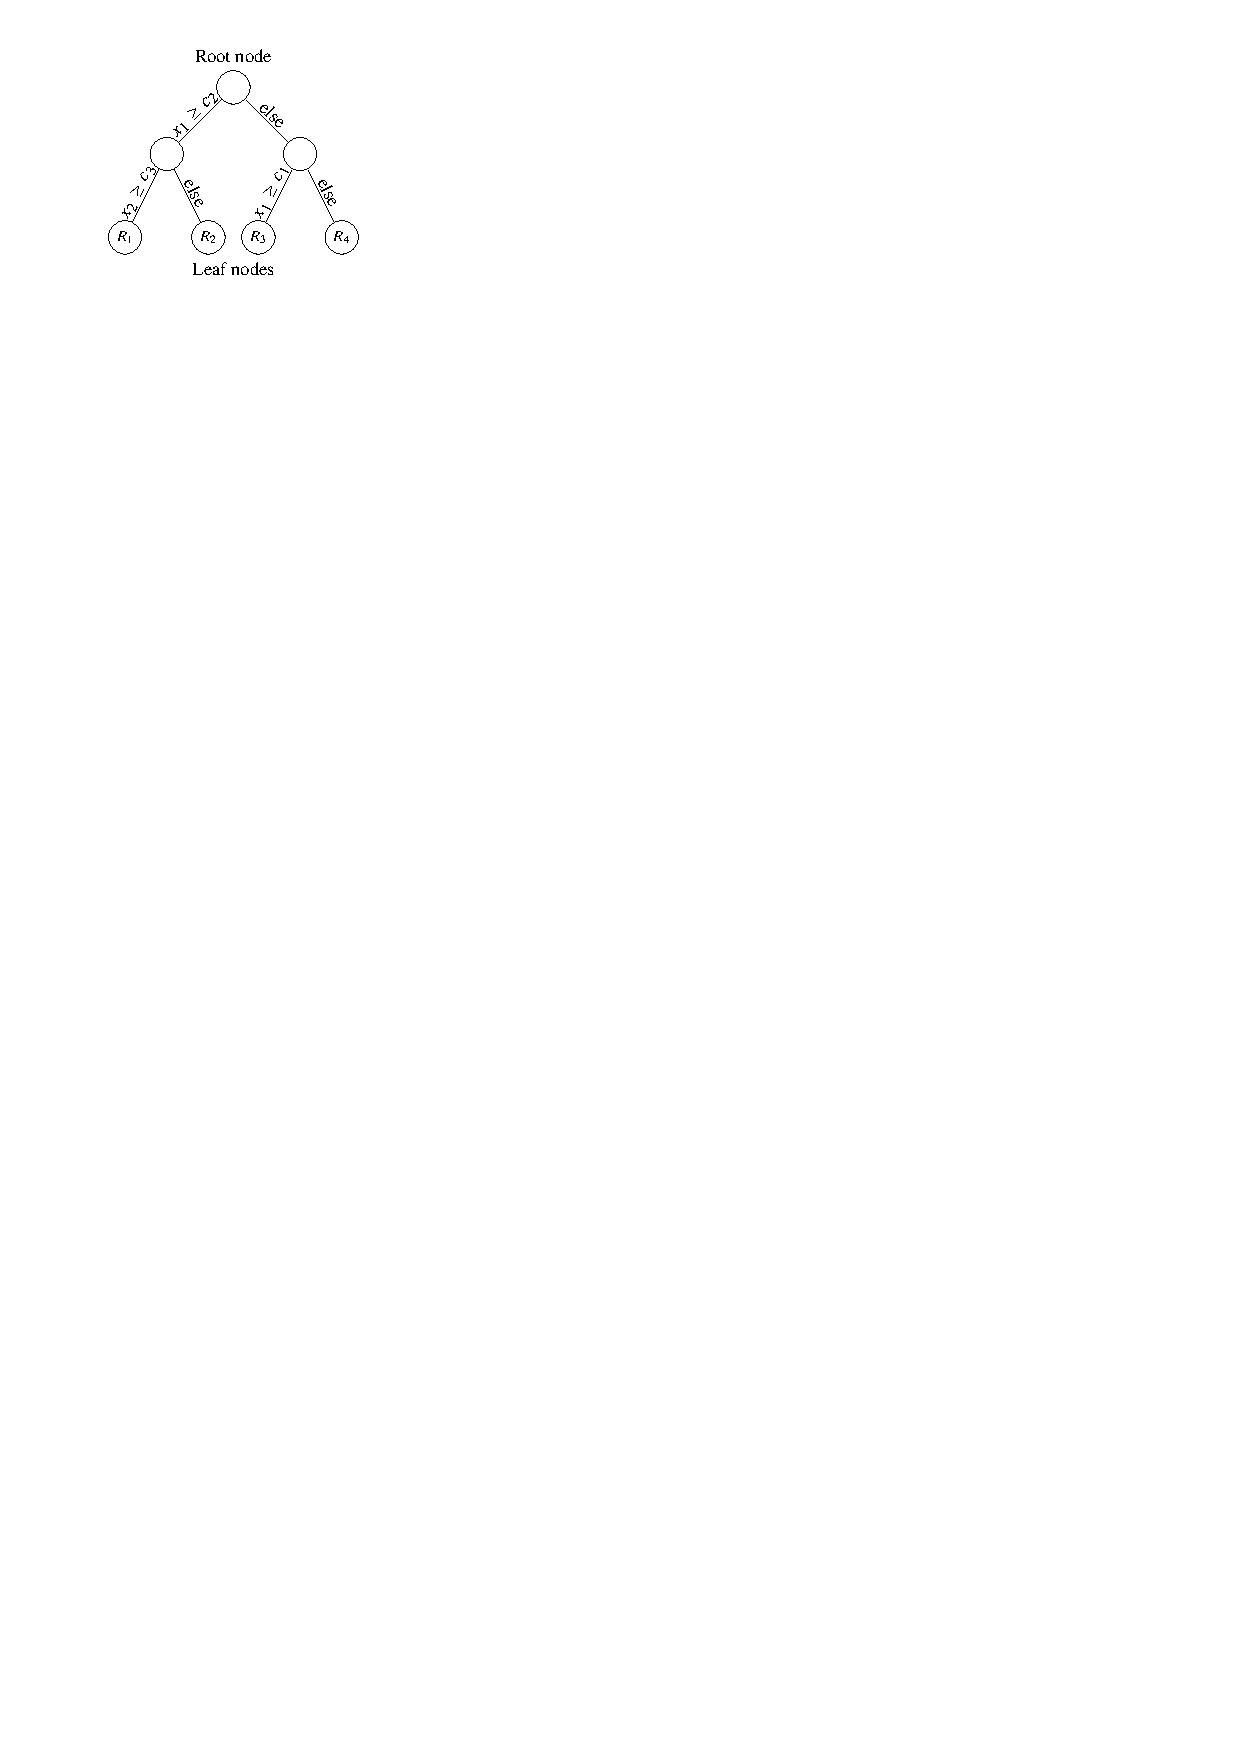
\includegraphics[scale=1.05]{ml/decision_tree}
    \subcaption{Binary tree structure of a decision tree.}
  \end{subfigure}\hfill%
  \begin{subfigure}[b]{0.46\textwidth}
    \centering
    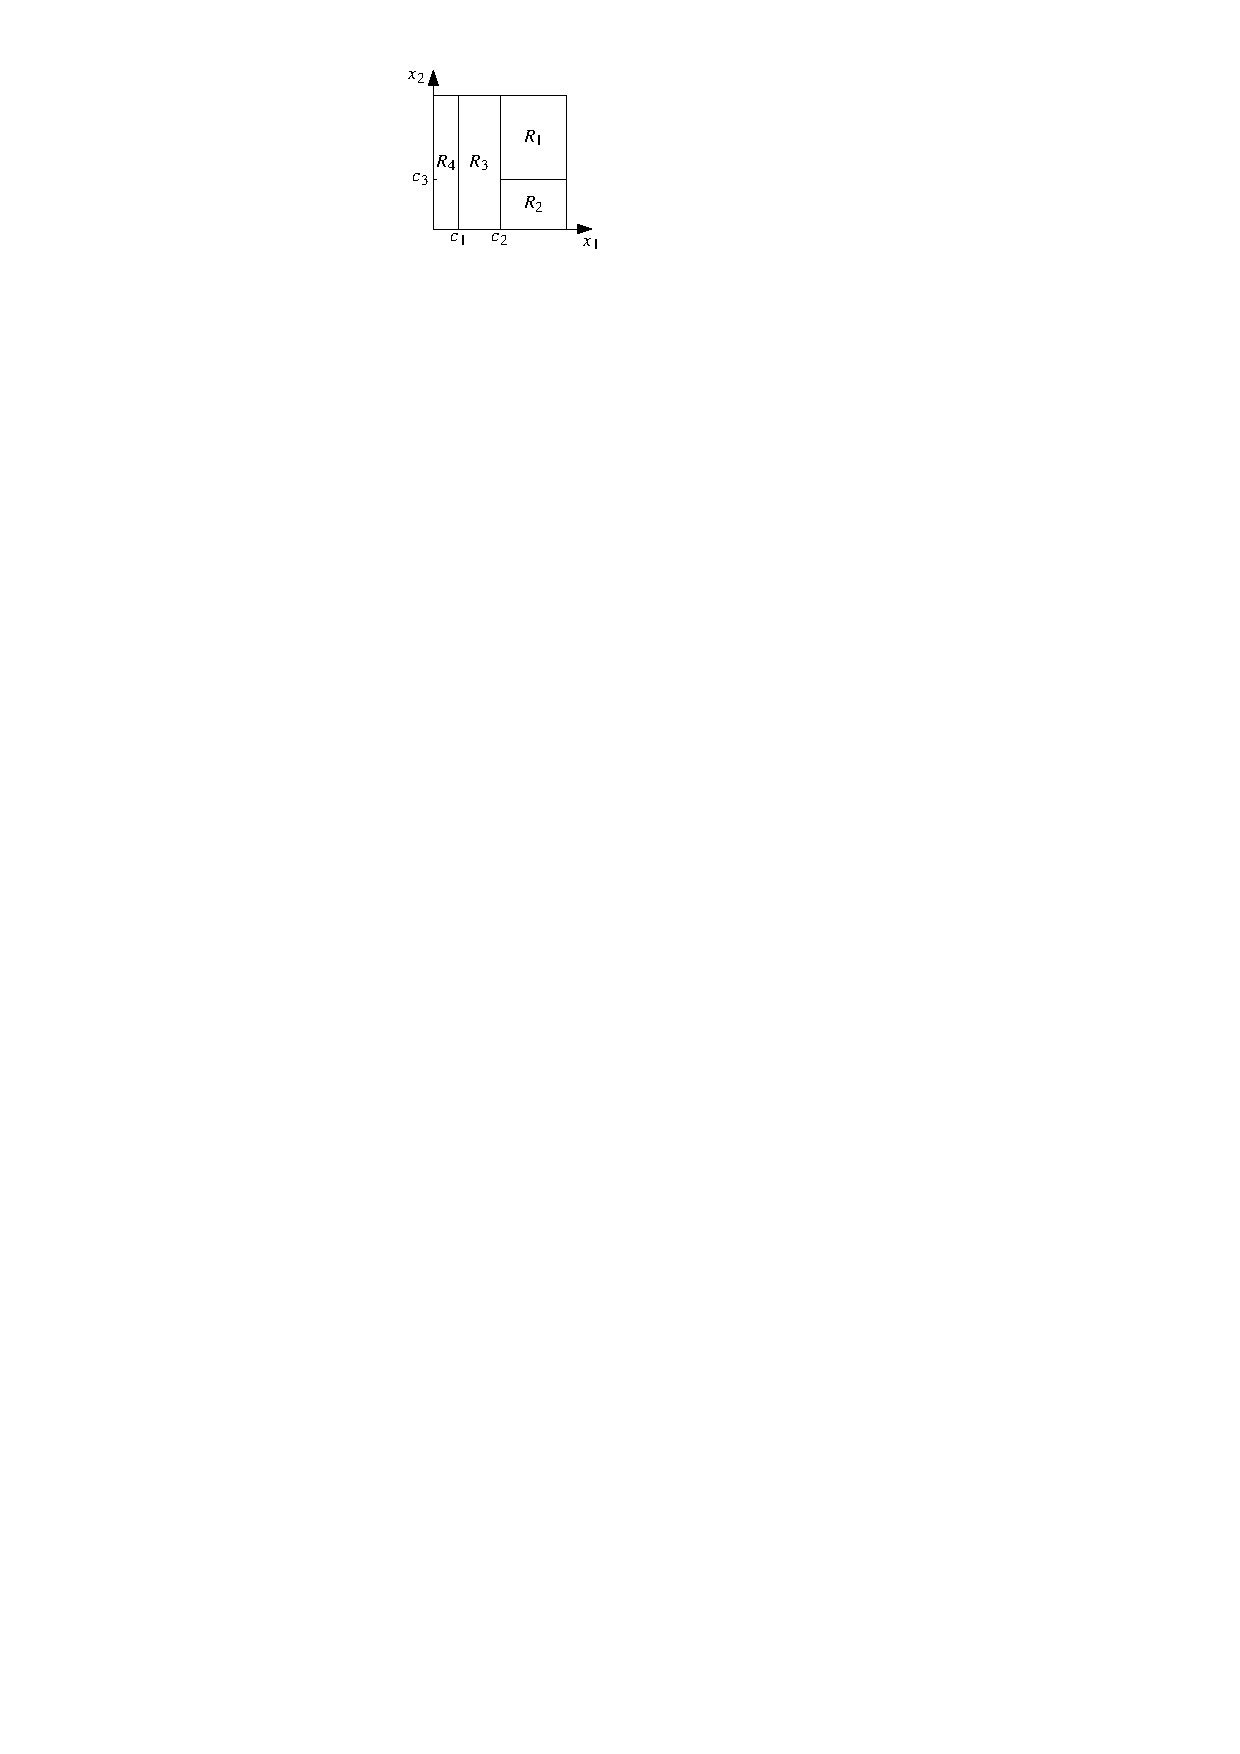
\includegraphics[scale=1.05]{ml/decision_tree_partitioning}
    \vspace*{0.7em}
    \subcaption{The partitioning resulting from the binary tree in (a).}
  \end{subfigure}\hfill%

  \caption[Example of a decision tree partitioning a two-dimensional
  space.]{Example of a decision tree partitioning a two-dimensional space with
    coordinates~$(x_1, x_2)$. The tree has a depth of two and four leaf nodes
    that define the regions~$R_1, \dots, R_4$. The figure is adapted from
    Ref.~\cite{hastie09}.}%
  \label{fig:decision_tree}
\end{figure}

% The construction of decision trees for regression (regression trees) is
% summarised hereafter.
The construction of regression trees is summarised hereafter. First, constraints
are set on the tree structure as a means to limit tree complexity, for example
by setting a maximum tree depth.
%The following steps are assumed to be subject to the chosen constraints.
In the ideal case, regression trees are constructed by finding a
partitioning~$\{R_j\}_{j=1}^{J}$ and leaf node constants~$\{c_j\}_{j=1}^{J}$
that minimise the mean squared error (MSE) given by
\begin{align*}
  \text{MSE} = \frac{\sum_{i = 1}^{N} w_i \left( y_i - h\bigl( \myvec{x}_i; \{c_j, R_j\}_{j=1}^{J} \bigr) \right)^2}{\sum_{i = 1}^{N} w_i} \,\text{,}
\end{align*}
where~$\{ (\myvec{x}_i, y_i, w_i) \}_{i=1}^{N}$ is a sample of training data
with scalar targets~$y_i$ and sample weights~$w_i$. Generally, this optimisation
problem is not easily solved; therefore, a greedy tree growth strategy is used
instead~\cite{james2013introduction,hastie09}. At any stage of the tree growing
algorithm, the split (and the corresponding leaf node constants) leading to the
largest reduction in MSE is chosen. The tree growing algorithm terminates once
no further splits can be performed.

% Consider a candidate split of a parent node (P) into a left (L) and right (R)
% daughter node. Let~$(y, w)$ be the tuple of regression target and weight for a
% given training example. Moreover, let $T_{\text{P}}$, $T_{\text{L}}$, and
% $T_{\text{R}}$ denote the set of $(y, w)$ for training examples populating the
% parent node, left daughter node, and right daughter node, respectively. The
% reduction in MSE by the candidate split is given by
% \begin{align*}
%   \Delta\text{MSE} =
%   \frac{1}{\sum_{i = 1}^{N} w_i} \left(
%   \sum_{(y, w) \in T_{\text{P}}} w (y - c_{\text{P}})^2
%   - \sum_{(y, w) \in T_{\text{L}}} w (y - c_{\text{L}})^2
%   - \sum_{(y, w) \in T_{\text{R}}} w (y - c_{\text{R}})^2
%   \right) \,\text{,}
% \end{align*}
% where the leaf node constants minimising the MSE criterion are given by
% \begin{align*}
%   c_{i} = \frac{ \sum_{(y, w) \in T_{i}} w y }{ \sum_{(y, w) \in T_{i}} w }
% \end{align*}
% for $i = \text{P}, \text{L}, \text{R}$~\cite{Breiman:1984jka,hastie09}.


% The tree growing terminates once no splits can be performed

% Classification trees are constructed with the goal that the partitioning of
% the input space yields subregions with low impurity, that is, the regions are
% mostly populated by training examples of a single class. In this case, the
% impurity of a tree node is quantified by the Gini index
% \begin{align*}
%   I_{\text{G}}(p) = 2 p (1 - p) \,\text{,}
% \end{align*}
% where $p$ is the proportion of examples from the positive class in a given
% node~\cite{hastie09}. A \emph{greedy} strategy is adopted to grow decision
% trees by performing the best possible split at every node. This split is
% determined by minimising the weighted sum of Gini impurities of the resulting
% daughter nodes, where impurities are weighted according to the total weight of
% training examples populating a given node. In the classification case, the
% constants $c_j$ assigned to leaf nodes of the tree are either--depending on
% the algorithm configuration--the proportion of examples from the positive
% class or the class label of the majority class in a given leaf node.


\subsubsection{Boosting of Decision Trees}

Boosting is an approach of solving prediction tasks by constructing models of
the form
\begin{align*}
  F_{M}\bigl(\myvec{x}; \{ \beta_m, \gamma_{m} \}_{m=1}^{M} \bigr) = \sum_{m = 1}^{M} \beta_m b(\myvec{x}; \gamma_{m}) \,\text{,}
\end{align*}
where $\beta_m$ are coefficients and $b(\myvec{x}; \gamma_{m})$ are basis
functions parameterised
by~$\gamma_{m}$~\cite{Friedman:2000,Friedman:2001wbq}. While there is some
flexibility in choosing the family of basis functions, boosting is typically
applied to decision trees.
% Given a sample of training data, the model is fit using an
% iterative procedure in which the $m$-th stage of the model, which is given by
% \begin{align*}
%   F_{m}\bigl(\myvec{x}; \{ \beta_{n}, \gamma_{n} \}_{n=1}^{m} \bigr) = F_{m - 1}\bigl( \myvec{x}; \{ \beta_{n}, \gamma_{n} \}_{n=1}^{m-1} \bigr) + \beta_m b(\myvec{x}; \gamma_{m}) \,\text{,}
% \end{align*}
% is determined by choosing $\beta_{m}$ and $\gamma_{m}$ such that an objective
% function is improved~\cite{hastie09}. Notably, the $m$-th stage does not alter
% the parameters~$\{ \beta_{n}, \gamma_{n} \}_{n=1}^{m-1}$.
The following is concerned with a boosting algorithm called gradient
boosting~\cite{Friedman:2001wbq}. Gradient boosting is particularly versatile,
as it constructs models by minimising an arbitrary differentiable loss function.
This allows gradient boosting to be applied to various kinds of prediction
tasks, an example of binary classification being given hereafter.

% The following\todo{Should say that there are other algorithms.} is concerned
% with a boosting algorithm referred to as gradient
% boosting~\cite{Friedman:2001wbq}. Gradient boosting is an algorithm for
% constructing additive models that minimise arbitrary differentiable loss
% functions, thus making it a useful tool for solving various prediction tasks.

Consider a binary classification problem with predictors~$\myvec{X}$ and class
labels~$Y$, which are $Y = +1$ for the positive class and $Y = -1$ for the
negative class.
% Both $\myvec{X}$ and $Y$ are random variables.
Further, let
\begin{align}
  L(Y, F(\myvec{X})) = \ln\mathopen{}\left(
  1 + e^{-Y F(\myvec{X})}
  \right)\mathclose{}
  \label{eq:loss_gradboost}
\end{align}
be a loss function and $F$~be a scalar function of the predictors. The function
that minimises the expected loss is given by
\begin{align*}
  F^{*\!}(\myvec{x})
  = \argmin_F \, \expect[ L(Y, F) \mid \myvec{X} = \myvec{x} ]
  = \ln\mathopen{}\left(
  \frac{
  \mathbb{P}(Y = +1 \mid \myvec{X} = \myvec{x})
  }{
  \mathbb{P}(Y = -1 \mid \myvec{X} = \myvec{x})
  }
  \right)\mathclose{} \,\text{,}
  %\label{eq:gradboost_logodds}
\end{align*}
which are the conditional log-odds of an observation with predictors~$\myvec{x}$
belonging to the positive class~\cite{Friedman:2000}. Knowledge of $F^{*\!}$
would solve the classification task since
\begin{align}
  \mathbb{P}(Y = +1 \mid \myvec{X} = \myvec{x}) = \frac{1}{1 + e^{-F^{*\!}(\myvec{x})}}
  \qquad \text{and} \qquad
  \mathbb{P}(Y = -1 \mid \myvec{X} = \myvec{x}) = \frac{1}{1 + e^{+F^{*\!}(\myvec{x})}} \,\text{,}
  \label{eq:gradboost_probas}
\end{align}
thus motivating the choice of loss function in \Cref{eq:loss_gradboost} for
binary classification.

An algorithm referred to as \textsc{TreeBoost} proposed by
Friedman~\cite{Friedman:2001wbq} is outlined. \textsc{TreeBoost} uses gradient
boosted decision trees and the loss function in \Cref{eq:loss_gradboost} to fit
a binary classifier to a sample of training data. A version of this algorithm is
employed in \textsc{TMVA}~\cite{TMVA}, which provides the BDT implementation
used in this thesis. The description is adapted from
Ref.~\cite{Friedman:2001wbq} with some modifications.
% (e.g.\ allowing training data to be weighted).

\vspace{11pt}
\noindent\textbf{\textsc{TreeBoost} algorithm for binary classification}
\nopagebreak\\[11pt]\nopagebreak
\noindent Inputs:
\begin{itemize}[itemsep=2pt]
\item Training data $\{(\myvec{x}_i, y_i, w_i)\}_{i = 1}^{N}$ with
  predictors~$\myvec{x}_i$, class labels $y_i$, and weights~$w_i$.
\item Number of boosting iterations $M$.
\item Shrinkage parameter~$\eta$ ($0 < \eta \leq 1$).
\item Hyperparameters of the regression tree algorithm.
\end{itemize}

\vspace{6pt}
\noindent Algorithm:
\begin{enumerate}[itemsep=2pt]

\item The model is initialised to
  \begin{align*}
    F_0(\myvec{x}) = \ln\mathopen{}\left( \frac{1 + \bar{y}}{1 - \bar{y}}
    \right)\mathclose{}
    \qquad \text{with} \qquad
    \bar{y} = \frac{\sum_{i=1}^{N} w_i y_i}{\sum_{i=1}^{N} w_i} \,\text{,}
  \end{align*}
  which is the training sample estimate of the (unconditional) log-odds of
  $Y = +1$.

\item For $m = 1$ to $M$:
  \begin{enumerate}[itemsep=2pt]

  \item Calculate the pseudo-residual
    \begin{align*}
      r_i
      = - \left. \frac{\partial L(y_i, F(\myvec{x}_i))}
      {\partial F(\myvec{x}_i)}\right|_{F(\myvec{x}_i) = F_{m - 1}(\myvec{x}_i)}
      \overset{\text{Eq.\ (\ref{eq:loss_gradboost})}}{=}
      %\frac{y_i}{1 + \exp(y_i F_{m-1}(\myvec{x}_i))}
      \frac{y_i}{1 + e^{y_i F_{m-1}(\myvec{x}_i)}}
    \end{align*}
    for all training examples.

  \item Fit a regression tree to estimate the relationship between
    pseudo-residuals and predictors using
    $\{(\myvec{x}_i, r_i, w_i)\}_{i = 1}^N$ as the training dataset. The
    prediction of the fitted regression tree is denoted by
    $h\bigl( \myvec{x}; \{c_{jm}, R_{jm}\}_{j=1}^{J_{m}} \bigr)$, where $J_{m}$
    is the number of leaf nodes, $c_{jm}$ is the constant predicted by the
    $j$-th leaf node, and $R_{jm}$ is the region defined by the $j$-th leaf
    node.

  \item The leaf node constants of the regression tree,
    $\{c_{jm}\}_{j=1}^{J_{m}}$, are updated to minimise
    \begin{align*}
      \sum_{i=1}^{N} w_i \cdot
      L\mathopen{}\left( y_i, F_{m - 1}(\myvec{x}_i)
      + h\bigl( \myvec{x}_i; \{c_{jm}, R_{jm}\}_{j=1}^{J_{m}} \bigr)
      \right)\mathclose{}
      \,\text{.}
    \end{align*}
    This optimisation problem has no analytical minimiser for the loss function
    in \Cref{eq:loss_gradboost}. Instead, the $\{c_{jm}\}_{j=1}^{J_{m}}$ are
    chosen to approximately minimise the above criterion by performing a single
    step of Newton's method.
    % \footnote{The starting point for Newton's method is taken to be
    % $c_{jm} = 0$ for all leaf nodes.}
    This yields the updated leaf node constants
    \begin{align*}
      c_{jm}^\prime = \frac{ \sum_i w_i r_i }{ \sum_i w_i |r_i| (1 - |r_i|)} \,\text{,}
    \end{align*}
    where the sums go over the training data populating the $j$-th leaf node of
    the tree. This step is specific to the \textsc{TreeBoost} algorithm by
    Friedman.

  \item Determine the $m$-th stage of the model by setting
    \begin{align*}
      F_m(\myvec{x}) = F_{m - 1}(\myvec{x})
      + \eta \cdot h\bigl( \myvec{x}; \{c_{jm}^\prime, R_{jm}\}_{j=1}^{J_{m}} \bigr)
      \,\text{,}
    \end{align*}
    where $\eta$ is a parameter of the boosting algorithm referred to as the
    \emph{shrinkage} or \emph{learning rate}. Generally, the shrinkage is set to
    values below unity such that every stage of boosting performs a suboptimal
    update. This serves as a form of regularisation to prevent overfitting.

  \end{enumerate}

\item The final prediction of the boosting procedure,
  $F_{M\hspace{-0.07em}}(\myvec{x})$, can be used to estimate the probability
  $\mathbb{P}(Y = +1 \mid \myvec{X} = \myvec{x})$ according to
  \Cref{eq:gradboost_probas} as
  \begin{align*}
    p(\myvec{x}) = \frac{1}{1 + e^{-F_{M\hspace{-0.07em}}(\myvec{x})}} \,\text{.}
  \end{align*}
  In HEP, this quantity is often referred to as the \emph{BDT score}.

\end{enumerate}
This algorithm is reminiscent of the classical gradient descent algorithm for
minimisation. However, in the case of gradient boosting the optimisation is
performed in the space of functions and not in parameter
space~\cite{Friedman:2001wbq}. Steps~2a) and 2b) of the algorithm estimate the
negative gradient of the loss function with respect to~$F(\myvec{x})$, which is
evaluated at the function estimate of the previous boosting iteration. Classical
gradient descent algorithms sometimes determine the step size of the parameter
update by performing a line search along the direction of steepest descent. In
the \textsc{TreeBoost} algorithm, this step size is determined by step 2c) on a
per-leaf basis.
% , however, for \textsc{TreeBoost} the size of the gradient descent step is
% determined on a per-leaf basis.
Finally, step 2d) performs the (regularised) gradient descent update.


\subsection{Neural Networks}%
\label{sec:neural_networks}

Neural networks (NNs) are parametric functions defined by the composition of
multiple, generally non-linear, functions. The functions composing NNs are also
referred to as \emph{layers}. An illustrative example of an NN is the
\emph{multilayer perceptron} (MLP). The basic element of MLPs, and many other
types of NNs, are \emph{densely connected layers} that apply transformations of
the form
\begin{align*}
  \myvec{f}_i(\myvec{x}; \myvec{W}_i, \myvec{b}_i) = \myvec{\phi}_i(\myvec{W}_i \myvec{x} + \myvec{b}_i) \,\text{,}
  % \label{eq:dense_layer}
\end{align*}
where $\myvec{x}$ is the layer input, $\myvec{W}_i$ and $\myvec{b}_i$ is a
weight matrix and bias vector, respectively, and $\myvec{\phi}_i$ is an
activation function that is applied element-wise.\footnote{The element-wise
  application of a function~$f(x)$ on a vector~$\myvec{x} = (x_1, \dots, x_n)$
  is defined as $\myvec{f}(\myvec{x}) = \bigl( f(x_1), \dots, f(x_n) \bigr)$.}
An MLP with $N$~hidden layers is defined by the composition of $N + 1$ densely
connected layers, yielding the expression
\begin{align*}
  \myvec{f}\bigl( \myvec{x}; \{\myvec{W}_{i},\myvec{b}_{i} \}_{i=1}^{N+1} \bigr)
  = \bigl( \myvec{f}_{N+1} \circ \dots \circ \myvec{f}_{1} \bigr)
  \bigl( \myvec{x}; \{\myvec{W}_i, \myvec{b}_i\}_{i=1}^{N+1} \bigr)
\end{align*}
for the MLP output. In general, the structure of NNs can be more complex than
illustrated in this example. Therefore, NN architectures are frequently
expressed as directed graphs with nodes representing layers and edges defining
how layers are composed.

% For the MLP example, this graph is
% \begin{align*}
%   (\myvec{x} \to) \, \text{Dense}_{1} \to \dots \to \text{Dense}_{N + 1}
% \end{align*}
% where $\text{Dense}_{i}$ denotes the $i$-th densely connected layer, and
% $\myvec{x}$ represents the input to the MLP. The $(N+1)$-th densely connected
% layer is also referred to as the output layer.

NNs are able to approximate large classes of
functions~\cite{cybenko1989approximation,hornik1989multilayer}, making them
attractive candidates for machine learning applications.
% Hereafter, the prediction of a generic NN with a is denoted by
% $f(\myvec{x}; \myvec{\theta})$, where $\myvec{x}$ is the NN input and
% $\myvec{\theta}$ are its parameters.
Consider a binary classification problem with predictors~$\myvec{X}$ and class
labels~$Y$, which take values of $Y = 1$ and $Y = 0$ for the positive and
negative class, respectively. Moreover,
let~$f(\myvec{x}; \myvec{\theta}) \in (0, 1)$ denote the prediction of an NN
with inputs~$\myvec{x}$ and free parameters~$\myvec{\theta}$.\footnote{Using the
  logistic (sigmoid) function as the activation function of the final layer
  constrains NN outputs to be within $(0, 1)$.} In this case, the canonical loss
function for binary classification is
\begin{align}
  L(Y, f(\myvec{X}; \myvec{\theta})) =
  \begin{cases}
    -\ln\mathopen{}\left( f(\myvec{X}; \myvec{\theta}) \right)\mathclose{},       & Y = 1 \\
    -\ln\mathopen{}\left( 1 - f(\myvec{X}; \myvec{\theta}) \right)\mathclose{},   & Y = 0 \\
  \end{cases} \,\text{,}
  \label{eq:loss_bce}
\end{align}
% where it is assumed that the NN can be defined such that
% $f(\myvec{x}, \myvec{\theta}) \in (0, 1)$, for example by using the logistic
% (sigmoid) function as the activation function in the final layer.
which is called the \emph{binary cross-entropy loss}. The function that
minimises the expected binary cross-entropy loss is
\begin{align*}
  f^{*\!}(\myvec{x})
  = \argmin_{f} \expect[ L(Y, f) \mid \myvec{X} = \myvec{x} ]
  = \mathbb{P}(Y = 1 \mid \myvec{X} = \myvec{x}) \,\text{,}
\end{align*}
motivating the use of \Cref{eq:loss_bce} as a loss function for binary
classification.
% This footnote is probably not needed.
%
% \footnote{The loss function in \Cref{eq:loss_bce} is similar to the one used
% for binary classification with gradient boosted trees in
% \Cref{eq:loss_gradboost}. This is due to both being derived from the negative
% log-likelihood of the Bernoulli distribution (the distribution of $Y$). The
% only differences are the change in class labels ($Y \in \{-1, 1\}$ for boosted
% trees; $Y \in \{0, 1\}$ for NNs) and the fact that the ensemble of trees
% approximates the conditional log-odds of $Y = 1$ while the NN estimates the
% conditional probability of $Y = 1$, directly.}

The binary classification task can be solved by approximating
$f^{*\!}(\myvec{x})$ using an NN with parameters set such that the mean loss
over a sample of training data~$\{ (\myvec{x}_i, y_i, w_i) \}_{i = 1}^N$ is
minimised. Formally, the parameters are given by the optimisation problem
\begin{align*}
  \myvec{\hat{\theta}} =
  \argmin_{\myvec{\theta}}\mathopen{}\left(
  \frac{\sum_{i = 1}^{N} w_i L(y_i, f(\myvec{x}_i; \myvec{\theta}))}{\sum_{i = 1}^{N} w_i}
  \right)\mathclose{}
  \,\text{.}
\end{align*}
This optimisation is non-convex and analytically intractable (for non-trivial
NNs). In practice, the minimisation is often performed using \emph{stochastic
  gradient descent} (SGD) or derivatives thereof. SGD is a gradient-based
optimisation method in which the gradient of the loss function is estimated
using random subsamples of training data. These subsamples are referred to as
\emph{mini-batches} and are denoted by
$\{\myvec{x}_{(i)}, y_{(i)}, w_{(i)}\}_{i=1}^{M}$ for a batch of size
$M$~\cite{Goodfellow-et-al-2016}. The mini-batch estimate of the gradient is
given by
\begin{align*}
  \myvec{g}(\myvec{\theta})
  = \frac{
  \sum_{i=1}^{M} w_{(i)}  \nabla_{\!\myvec{\theta}} L(y_{(i)}, f(\myvec{x}_{(i)}; \myvec{\theta}))
  }{
  \sum_{i=1}^{M} w_{(i)}
  } \,\text{,}
\end{align*}
where $\nabla_{\!\myvec{\theta}}$ refers to the vector of partial derivatives in
parameter space~\cite{Goodfellow-et-al-2016}. The training of NNs using SGD
proceeds by first randomly initialising the parameters to
$\myvec{\theta} = \myvec{\theta}_0$. Afterwards, a number of SGD iterations are
performed until convergence or another stopping criterion is met. The iterations
consist of drawing a mini-batch from the training data, computing the mini-batch
estimate of the gradient, and then performing the parameter update
\begin{align*}
  \myvec{\theta}_{t + 1} = \myvec{\theta}_{t} - \eta_{t} \myvec{g}(\myvec{\theta}_{t}) \,\text{,}
\end{align*}
where $\eta_{t}$ is referred to as the learning
rate~\cite{Goodfellow-et-al-2016}. The learning rate can follow a predefined
schedule with respect to the iteration counter~$t$, common ones being constant
or exponentially decaying learning rates. A modification of this algorithm is
\emph{SGD with momentum}, which aims to improve the convergence properties of
SGD~\cite{polyak1964some,rumelhart1986learning,sutskever2013importance}. The
modified algorithm alters the parameter update according to
\begin{align*}
  \myvec{\theta}_{t + 1} = \myvec{\theta}_{t}
  + \alpha \Delta\myvec{\theta}_{t} - \eta_t \myvec{g}(\myvec{\theta}_{t})
  \qquad \text{with} \qquad
  \Delta\myvec{\theta}_{t} =
  \begin{cases}
    \myvec{\theta}_{t} - \myvec{\theta}_{t - 1}, & t > 0 \\
    0,                                         & t = 0
  \end{cases}
\end{align*}
which introduces the momentum parameter
$0 \leq \alpha < 1$~\cite{rumelhart1986learning,Goodfellow-et-al-2016}. The
update of SGD with momentum can be loosely interpreted as the movement of a
massive object through parameter space with two forces acting on the object: a
force proportional to~$-\myvec{g}(\myvec{\theta})$ and a friction-like force
proportional and opposed to the
velocity~$\Delta\myvec{\theta}_{t}$~\cite{Goodfellow-et-al-2016}.


\subsubsection{Recurrent Neural Networks}%
\label{sec:rnn}

An appealing feature of NNs is their ability to process various forms of
unstructured data (e.g.~graphical images, natural language, etc.) using
specialised network architectures. Among these architectures are \emph{recurrent
  neural networks} (RNNs), which operate on ordered, variable-length
sequences. Such sequences occur in many scenarios, an example being the
representation of sentences in natural language processing. In the context of
HEP, one might encode the properties of jets reconstructed in a particle
collision event as a variable-length sequence. Hereafter, sequences are denoted
by~$(\myvec{x}_{t})_{t = 1}^{N}$, where~$t$ is conventionally referred to as
\emph{time} or a \emph{time step}, $N$ is the length of the sequence, and
$\myvec{x}_{t}$ represents the feature vector associated with the $t$-th element
of the sequence. When including sequence data as inputs or outputs in NNs,
layers that describe mappings of the form
\begin{alignat*}{3}
  &\text{Many-to-many:}\,
  &&(\myvec{x}_{t})_{t = 1}^{N} &&\ra (\myvec{y}_{t})_{t = 1}^{M} \\
  &\text{Many-to-one:}\,
  &&(\myvec{x}_{t})_{t = 1}^{N} &&\ra (\myvec{y}_{1}) \\
  &\text{One-to-many:}\,
  &&(\myvec{x}_1)              &&\ra (\myvec{y}_{t})_{t = 1}^{M} \,\text{,}
\end{alignat*}
are of particular interest. Additionally, for certain machine learning tasks it
can be beneficial to exploit the context in which an element of the input/output
sequence occurs. These capabilities are provided by recurrent NN layers, which
are described in the remainder of this section. The focus of the following
description lies on the \emph{many-to-one} and \emph{many-to-many} ($N = M$)
cases.

% When performing such computations, it can often be useful to exploit the
% context in which an element of the input/output sequence occurs.  For example,
% it can be beneficial to include information regarding the first $t - 1$
% elements of a sequence when processing the $t$-th element.  These kinds of
% computations are the primary motivation for RNNs. This thesis is mostly
% concerned with the many-to-one and many-to-many ($N = M$) cases.

The ability of RNNs to perform computations involving variable-length sequences
while exploiting contextual information is enabled by two concepts:
\emph{parameter sharing} and the inclusion of an \emph{internal state} in the
network. These concepts are illustrated using the example of the \emph{long
  short-term memory} (LSTM) layer~\cite{lstm,gers2000learning}. Consider an
input and output sequence denoted by $(\myvec{x}_{t})_{t = 1}^{N}$ and
$(\myvec{y}_{t})_{t = 1}^{N}$, respectively, both sequences having the same
length. In addition, let $\myvec{y}_{0} = \myvec{0}$. An LSTM layer computes the
output sequence by iterating over time steps starting at $t = 1$. Three
quantities referred to as \emph{gate activations} are defined
as~\cite{Goodfellow-et-al-2016}
\begin{alignat*}{3}
  \myvec{f}_{t} &= \myvec{\sigma}\bigl(\myvec{U}^{\text{f}}  \myvec{x}_{t} &&+ \myvec{W}^{\text{f}}  \myvec{y}_{t - 1} &&+ \myvec{b}^{\text{f}}\bigr) \\
  \myvec{i}_{t} &= \myvec{\sigma}\bigl(\myvec{U}^{\text{i}}  \myvec{x}_{t} &&+ \myvec{W}^{\text{i}}  \myvec{y}_{t - 1} &&+ \myvec{b}^{\text{i}}\bigr) \\
  \myvec{o}_{t} &= \myvec{\sigma}\bigl(\myvec{U}^{\text{o}}  \myvec{x}_{t} &&+ \myvec{W}^{\text{o}}  \myvec{y}_{t - 1} &&+ \myvec{b}^{\text{o}}\bigr) \,\text{,}                                                       % \label{eq:lstm_gates}
\end{alignat*}
which are the gate activations of the \emph{forget gate}, \emph{input gate}, and
the \emph{output gate} at time $t$, respectively. The gate activations are
parameterised by weight matrices~$\myvec{U}^{\text{f/i/o}}$ and
$\myvec{W}^{\text{f/i/o}}$, as well as bias
vectors~$\myvec{b}^{\text{f/i/o}}$. For a given gate, the weights and biases are
the same for all time steps, which is an implementation of parameter sharing.
The function~$\myvec{\sigma}$ refers to the element-wise application of the
logistic (sigmoid) function, thus the components of the gate activation vectors
take values in $(0, 1)$. Moreover, an LSTM layer includes an internal state that
propagates and evolves forward through time. At time $t$, the state of an LSTM
is denoted by $\myvec{s}_{t}$, and the initial state is set to
$\myvec{s}_{0} = \myvec{0}$. The internal state of an LSTM at time $t$ is given
by the following recurrence relation~\cite{Goodfellow-et-al-2016,keras}
\begin{align}
  \myvec{s}_{t} = \myvec{f}_{t} \circ \myvec{s}_{t - 1}
  + \myvec{i}_{t} \circ \myvec{\phi}(\myvec{U} \myvec{x}_{t} + \myvec{W} \myvec{y}_{t-1} + \myvec{b}) \,\text{,}
  \label{eq:lstm_state_update}
\end{align}
where $\circ$ is the element-wise multiplication of two vectors, $\myvec{\phi}$
is an activation function defined by the element-wise application of the
hyperbolic tangent,\footnote{The choice of activation function in
  \Cref{eq:lstm_state_update} is specific to the implementation of LSTM networks
  in \textsc{Keras}~\cite{keras}.} and $\myvec{U}$, $\myvec{W}$, and $\myvec{b}$
are weights and biases shared across time steps. Finally, the output of the LSTM
layer at time~$t$ is given by~\cite{Goodfellow-et-al-2016}
\begin{align}
  &\myvec{y}_{t} = \myvec{o}_{t} \circ \myvec{\phi}(\myvec{s}_{t}) \,\text{,}
  \label{eq:lstm_output}
\end{align}
using the definitions introduced before.

The computational graph of an LSTM layer for a single time step is depicted in
\Cref{fig:lstm}, illustrating the role of the gates in controlling the flow of
information. The forget gate allows to selectively forget/remember aspects about
the internal state at time $t - 1$ by multiplying the state
vector~$\myvec{s}_{t - 1}$ by the activation of the forget gate. Similarly, the
input gate controls the inclusion of information derived from the current
element of the input sequence, $\myvec{x}_{t}$, and the output of the preceding
time step, $\myvec{y}_{t - 1}$, into the internal state at time~$t$. Lastly, the
output gate controls which parts of the internal state (after application of
$\myvec{\phi}$) are presented as the output~$\myvec{y}_{t}$. An input sequence
of length $N$ can be processed by repeating the computations depicted
in~\Cref{fig:lstm} until the input sequence is exhausted, thus yielding an
output sequence of the same length. Finally, a many-to-one mapping can be
achieved by discarding the first~$N - 1$ outputs of an LSTM and using
only~$\myvec{y}_{N}$ for further computation. A concrete example of LSTM layers
being used in HEP is given in \Cref{sec:tauid}.

\begin{figure}[htbp]
  \centering

  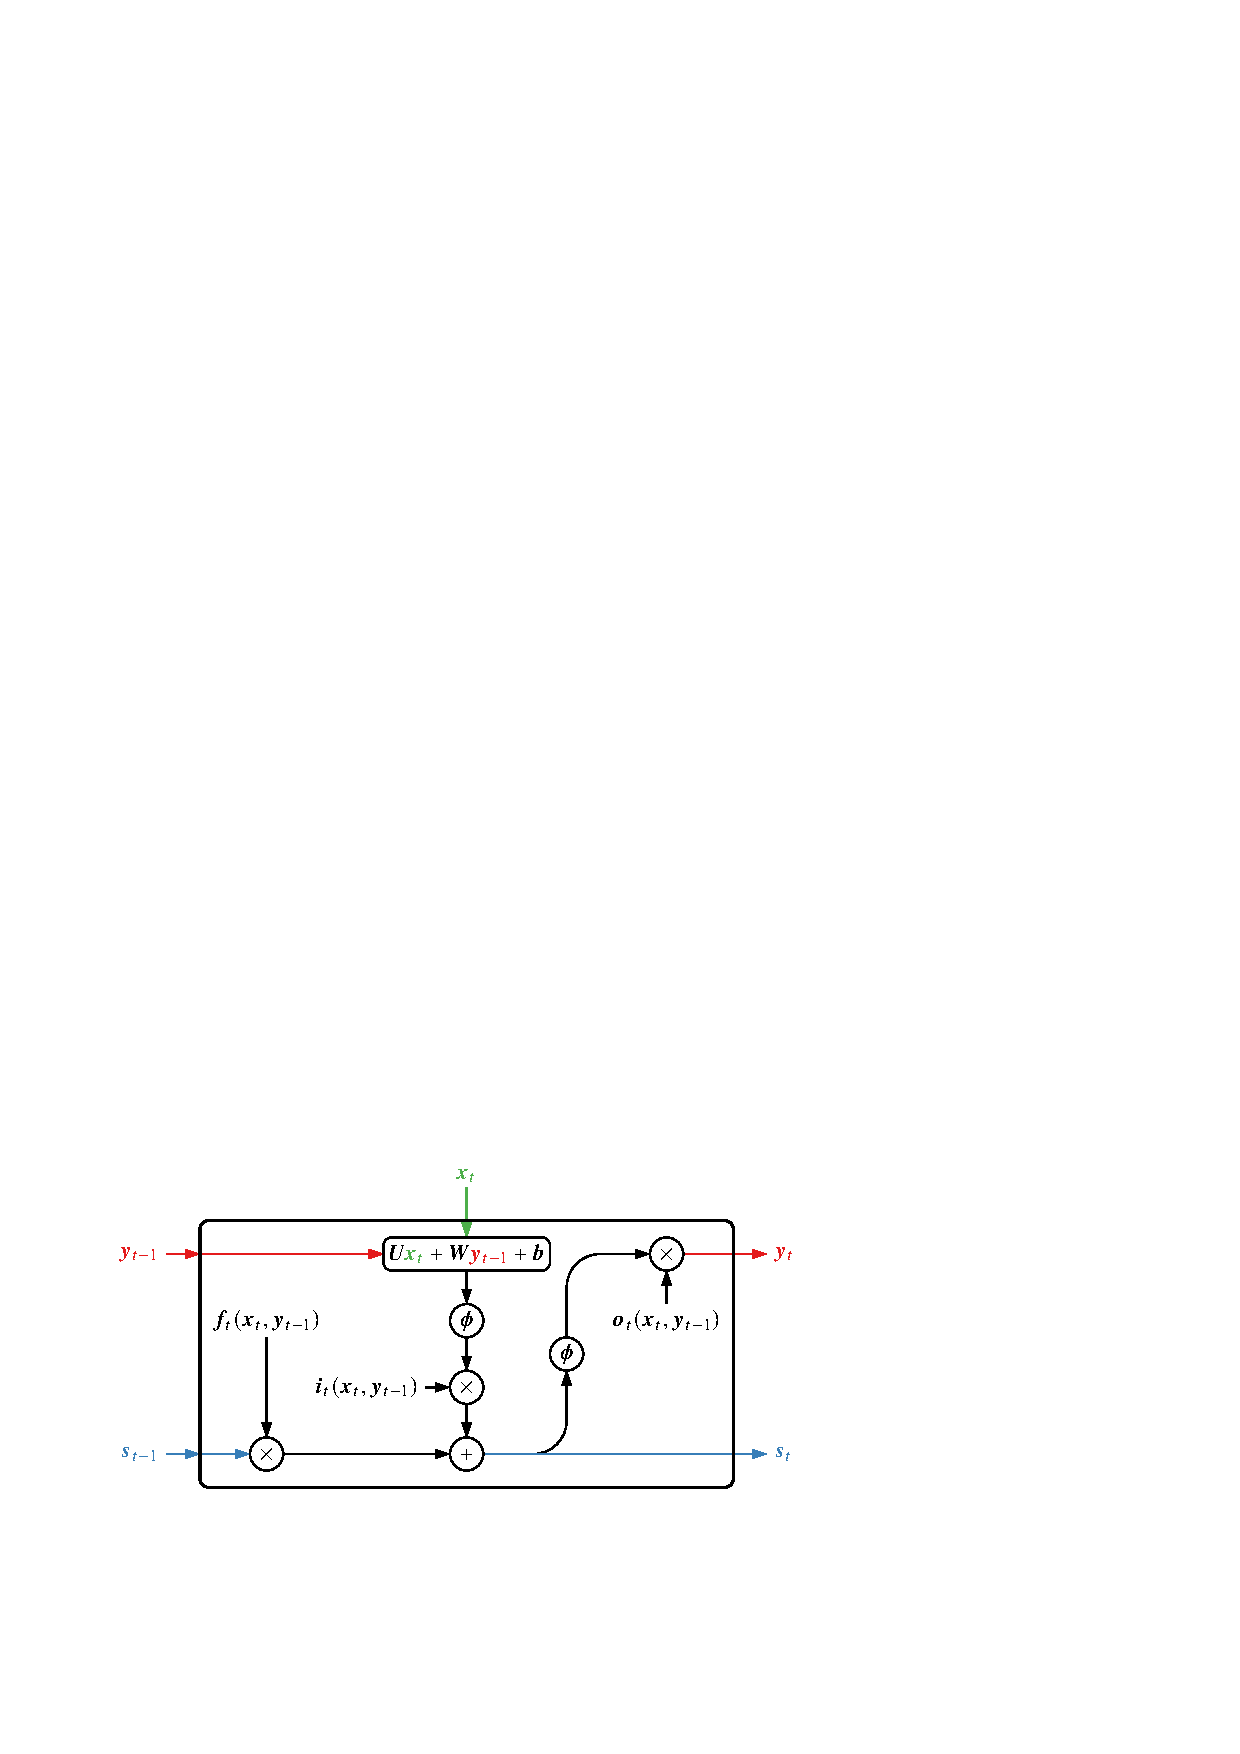
\includegraphics[scale=1.0]{ml/lstm}

  \caption[Computational graph of an LSTM layer.]{Computational graph of an LSTM
    layer for time step~$t$. Operations in circles represent element-wise
    multiplication ($\times$), element-wise addition ($+$), and element-wise
    application of the $\tanh$ activation function ($\myvec{\phi}$). The graph
    illustrates the computations performed as part of
    \Cref{eq:lstm_state_update,eq:lstm_output}. The computations involved in the
    calculation of the gate activation vectors are omitted, however, the
    dependency of the gate activation vectors on $\myvec{x}_{t}$ and
    $\myvec{y}_{t - 1}$ is indicated in parenthesis.}%
  \label{fig:lstm}
\end{figure}

% Alternatives to LSTM for processing ordered, variable-length sequences in NNs
% exist. For example, \emph{gated recurrent units}~\cite{cho2014properties} are
% recurrent layers similar to LSTM layers in the sense that they also exploit a
% gating mechanism to control the flow of information. A disadvantage of RNNs is
% the sequential nature of the computations they perform, thus preventing
% efficient parallelisation. Recently, a new architectures referred to as
% \emph{transformers}~\cite{vaswani2017attention} were introduced to address
% this problem.


%%% Local Variables:
%%% mode: latex
%%% TeX-master: "../../phd_thesis"
%%% End:
